\begin{frame}
\frametitle{Arquitectura del sistema}

\begin{itemize}
	\item<1-> \textcolor{UDCpink}{\itshape Front-end}: Creado en LÖVE, usa un modelo MVC que usa una interfaz gráfica en modo inmediato.
	
	\vspace{0.5em}
	
	\item<2-> \textcolor{UDCpink}{\itshape Back-end}: Creado en Lua 5.1 y ASP, usa un modelo en \textit{pipeline}.
	
\end{itemize}

\vspace{0.5em}

\pause[3]

\begin{center}
	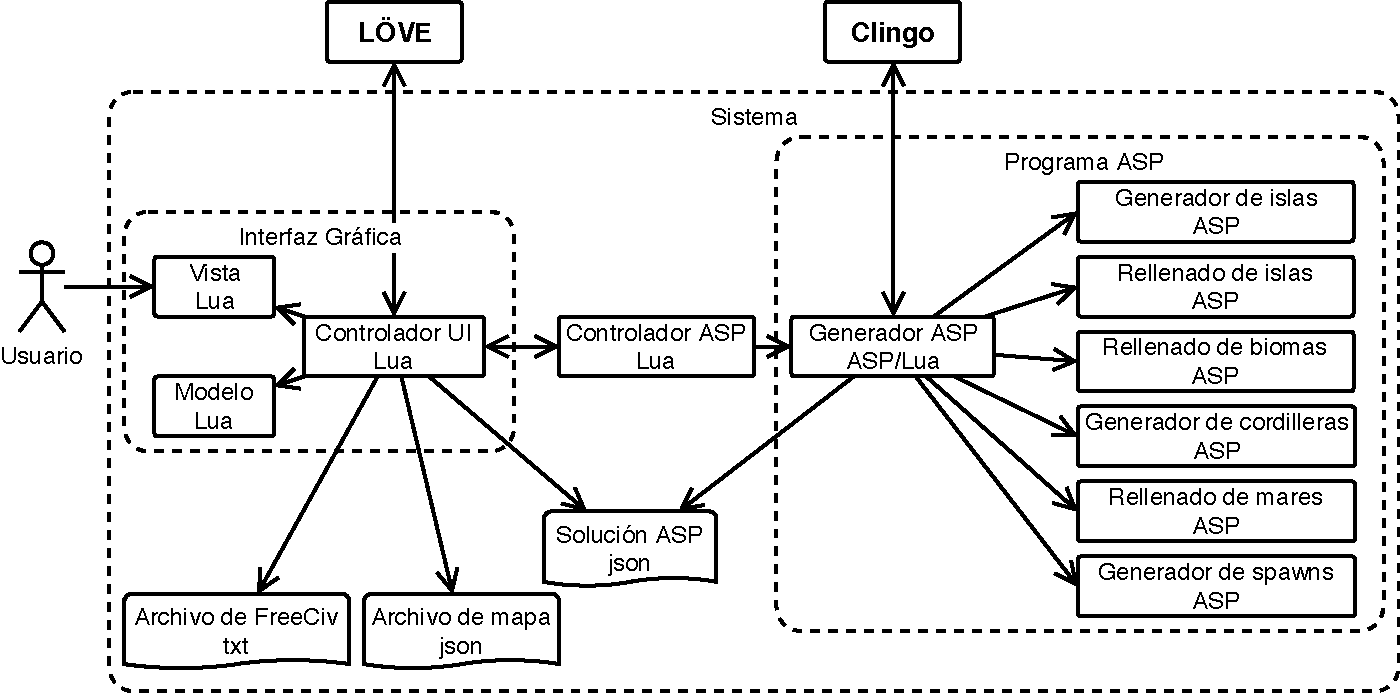
\includegraphics[width=0.7\textwidth]{images/arquitectura-completa.pdf}
\end{center}

\end{frame}

\begin{frame}
\frametitle{Proceso de ingeniería}

\begin{itemize}
	\item<1-> Metodología: \textcolor{UDCpink}{desarrollo iterativo incremental}.
	
	\vspace{0.5em}
	
	\item<2-> Se ha usado herramientas de \textcolor{UDCpink}{uso libre y gratuitas} para el desarrollo del proyecto.
	
	\vspace{0.5em}
	
	\item<3-> El coste total del proyecto asciende a \textcolor{UDCpink}{\EUR{3720.00}}.
	
	\vspace{1em}
	
	\pause[4]
	
	\begin{center}
		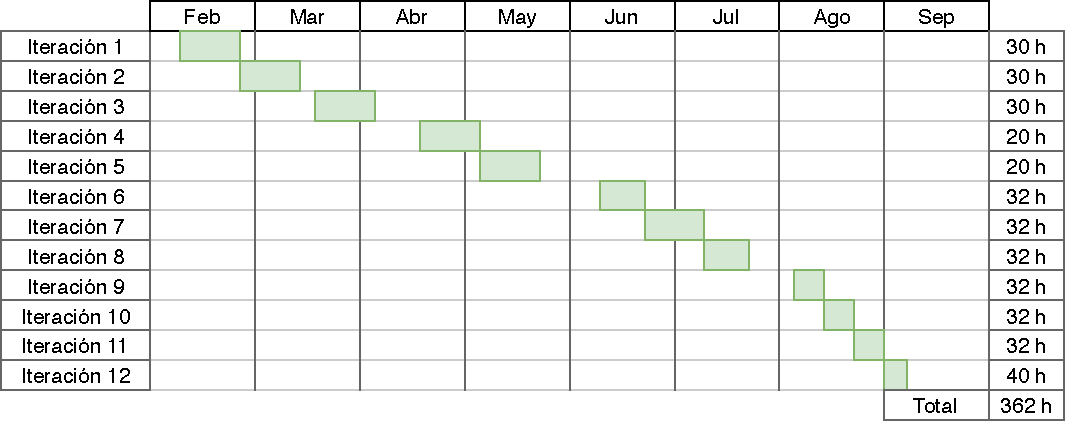
\includegraphics[width=0.85\textwidth]{images/gantt.pdf}
	\end{center}
	
\end{itemize}

\end{frame}